\documentclass{article}

\usepackage{../preamble}
\standalonetrue

\pagestyle{fancy}
\fancyhf{}
\rhead{Section \thesection}
\lhead{PHYS 304 Lecture 11}
\rfoot{Page \thepage}


\title{PHYS 304 Lecture 11}
\author{Ashtan Mistal}
\date{!!!}

\begin{document}

\ifstandalone
\maketitle
\fi

\graphicspath{{./Lecture11/}}

\section{Review of key points regarding the finite square well potential}


For the finite square well potential, there are a finite number of bound-to-the-well stationary state solutions of the SE for a discrete set of energies above the minimum potential in the well region.  They are bound because they are exponentially decaying outside of the well.

In the limit of an infinitely deep well, the energies of these bound states approach those we obtained earlier, but in general they differ, and must be obtained using a transcendental equation that is easy to solve “graphically”.  The transcendental equation is obtained using boundary conditions (continuity of the wavefunction and its derivative in the direction of propagation) to connect the solutions of the SE obtained separately in the 3 distinct spatial regions (made distinct by the potentials in those regions).

As the energy of these states approaches the surrounding potential, they become more and more delocalized in the barrier regions, but remain exponentially decaying.  As the energy goes above that in the barrier regions, the solutions of the SE in the barrier regions become sinusoidal, but with a different wavelength (or k value), for a given energy, than the sinusoidal solutions inside the well region.  Just like in the free electron case, there is no restriction on the energy above the barrier potentials, and the formal solutions to the SE, that consist of incident, reflected, and transmitted waves in the barrier regions, and backward and forward propagating waves in the well, are not normalizable.  These are referred to as “scattering states”, cf bound states. They are still very useful/relevant since one can form normalizable wavepackets out of them. \textbf{Can you guess what the dynamics of such wavepackets might be like?}

\subsection{Purpose of today's lecture}

...is to introduce new notation and review concepts from linear algebra in 2D real vector space using that new notation, so as to;

\begin{itemize}
    \item provide a reference point you can always go back to if you get confused using bra/ket notation in quantum mechanics
    \item emphasize the importance of being able to use arbitrary orthonormal bases to expand any QM “state”
    \item provide a very simple example of an “operator” that can be expanded in any basis
\end{itemize}

\section{Bra-ket notation applied to 2D real vectors}

Using 2D real vector space as a familiar example, where we assume some "fundamental", or "inertial" reference frame defined by unit vectors $\hat{\imath}$ and $\hat{\jmath}$, and using "bra and ket" notation to indicate the dotproduct operation: i.e. the dot product of two $2 \mathrm{D}$ real vectors $\vec{r}$ and $\vec{r}^{\prime}$, is denoted $\left\langle\vec{r}^{\prime} \mid \vec{r}\right\rangle$;

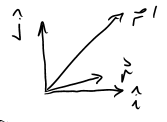
\includegraphics[width = 0.3 \textwidth]{Lecture11/1.png}

If $\braket{\hat{i} | \hat{\vec{r}'}} = x'$ and $\braket{j | \hat{\vec{r'}}} = y'$, the explicit vector associaited with ket $\ket{\vec{r'}}$ is:

$$\ket{\vec{r'}} \equiv \begin{bmatrix} x' \\ y' \end{bmatrix}$$

It thus follows that the explicit vector associated with $\bra{\vec{r'}}$ is:

$$\bra{\vec{r'}} \equiv \begin{bmatrix} x' & y' \end{bmatrix}$$

If you get rid of all the "primes", ', in the above, the corresponding explicit vectors associated with $|\vec{r}\rangle$ and $\langle\vec{r}|$ are:
$$
|\vec{r}\rangle=\left[\begin{array}{l}
x \\
y
\end{array}\right] \quad\langle\vec{r}|=[x, y]=\left[\begin{array}{l}
x \\
y
\end{array}\right]^{\text {Transpose }}
$$

Then the vector form of $\braket{\vec{r'} | \vec{r}}$ in terms of $x, y, x^{\prime}, y^{\prime}$ is:
$$
\left\langle\vec{r}^{\prime} \mid \vec{r}\right\rangle=\left[x^{\prime} y^{\prime}\right]\left[\begin{array}{l}
x \\
y
\end{array}\right]=x^{\prime} x+y^{\prime} y
$$

$$
\begin{aligned}
&\text { One can always write }|\vec{r}\rangle=[[\hat{i}\rangle(\hat{i}|+| \hat{j}\rangle \hat{i}|| \vec{r}) \text {. Proof: } \\
&\begin{aligned}
|\vec{r}\rangle &=\langle\hat{i} \mid \vec{r}\rangle|\hat{i}\rangle+\langle\hat{j} \mid \vec{r}\rangle|\hat{j}\rangle \\
\left[\begin{array}{l}
x \\
y
\end{array}\right] &\left.=\left(\left[\begin{array}{ll}
1 & 0
\end{array}\right]\left[\begin{array}{l}
x \\
y
\end{array}\right]\right)\left[\begin{array}{l}
1 \\
0
\end{array}\right]+\left(\begin{array}{ll}
[0 & 1
\end{array}\right]\left[\begin{array}{l}
x \\
y
\end{array}\right]\right)\left[\begin{array}{l}
0 \\
1
\end{array}\right] \\
&=x\left[\begin{array}{l}
1 \\
0
\end{array}\right]+y\left[\begin{array}{l}
0 \\
1
\end{array}\right]=\left[\begin{array}{l}
x \\
y
\end{array}\right]
\end{aligned}
\end{aligned}
$$

Why does this imply that $\ket{\hat{i}} \bra{i} + \ket{\hat{j}} \bra{\hat{j}}$ is a “unity operator” in 2D real vector space?

This is \textbf{not} a vector or number. It is a matrix, the identity matrix $\begin{pmatrix} 1 & 0 \\ 0 & 1 \end{pmatrix}$

$$\begin{pmatrix} 1 & 0 \\ 0 & 1 \end{pmatrix} = \begin{pmatrix} 1 & 0 \\ 0 & 0 \end{pmatrix} + \begin{pmatrix} 0 & 0 \\ 0 & 1 \end{pmatrix}$$

The latter two matrices being the projection operators. 

\section{Rotation Operator}

Assume that there is a different basis vector set, labelled $\left|\alpha_{1}\right\rangle$, and $\left|\alpha_{2}\right\rangle$, rotated by an angle $\phi$ with respect to the "fundamental" basis.

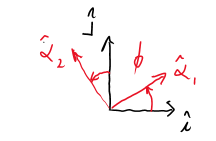
\includegraphics[width = 0.3 \textwidth]{Lecture11/2.png}

The unity operator in this new basis using bra ket notation is then:

$$\hat{I} = \ket{\hat{\alpha_1}} \bra{\hat{\alpha_1}} + \ket{\hat{\alpha_2}} \bra{\hat{\alpha_2}}$$

What are the components of $\ket{\hat{i}}$ and $\hat{\vec{j}}$ in this new basis?

$$\hat{\vec{i}} = \cos \phi \ket{\hat{\alpha_1}} - \sin \phi \ket{\hat{\alpha_2}}$$

$$\hat{\vec{j}} = \sin \phi \ket{\hat{\alpha_1}} + \cos \phi \ket{\hat{\alpha_2}}$$

Given an arbitrary vector $|\vec{r}\rangle$, how would you define an "operator", $\widehat{\mathrm{R}}(\theta)$ that would act on that vector and generate a new vector, $\left|\overrightarrow{r_{\theta}}\right\rangle$, that is rotated by an angle $\theta$ from the original direction of $|\vec{r}\rangle$, with the same magnitude; $\left|\overrightarrow{r_{\theta}}\right\rangle=\widehat{\mathrm{R}}(\theta)|\vec{r}\rangle$ ? Do this using the explicit vectors you defined in the "fundamental" basis for the two vectors, eg.
$$
\left[\begin{array}{l}
x_{\theta} \\
y_{\theta}
\end{array}\right]=[\hat{R}(\theta)]\left[\begin{array}{l}
x \\
y
\end{array}\right]
$$

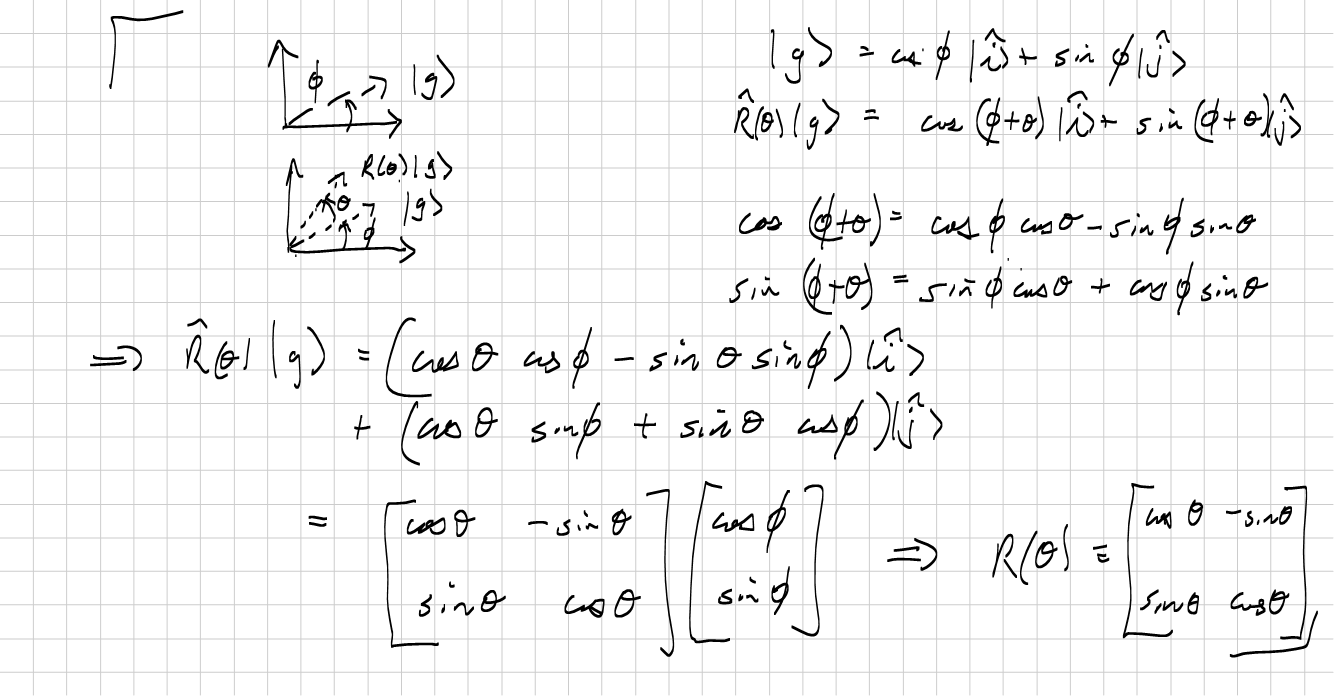
\includegraphics[width = 0.98 \textwidth]{Lecture11/3.png}

\subsection{Using arbitrary bases to evaluate immutable operations on immutable vectors}

How could you formally represent this 2D real vector rotation operation using bra and ket notation in an arbitrary basis $\ket{\hat{\alpha_1}}$, and $\ket{\hat{\alpha_2}}$?  Hint: insert the unity operator in the equation $\ket{\vec{r}_\theta} = \hat{R}(\theta) \ket{\vec{r}}$ and project onto that basis.  

$$\ket{\vec{r}_\theta} = \hat{R}(\theta) \ket{\vec{r}} = \hat{R} (\theta) \left( \sum_{j=1}^2 \ket{\hat{\alpha_j}} \bra{\hat{\alpha_j}} \right) \ket{\vec{r}}$$

$$\Rightarrow \braket{\hat{\alpha_j} | \vec{r}_\theta} = \sum_j \braket{\hat{\alpha_j} | \hat{R}(\theta) | \alpha_j} \left( \braket{\hat{\alpha}_j | \vec{r}} \right)$$

Just bra ket for matrix equation in that basis. 

\subsection{Matrix operators in different bases}

Interpret $\braket{\vec{\alpha_i} | \hat{R}(\theta) | \vec{\alpha_j}}$, and what explicitly are the matrix elements $\hat{R}(\theta)_{i,j}$?

\begin{itemize}
    \item Rotate basis vector $\ket{\hat{\alpha}_j}$ by $\theta$ and project onto $\ket{\hat{\alpha}_i}$
\end{itemize}

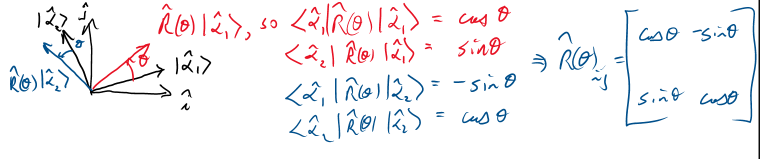
\includegraphics[width = 0.98 \textwidth]{Lecture11/4.png}






\end{document}